
\chapter{State of the Art and Literature Review}

This chapter will present the state of the art and literature review of the topics related to this project.
The topics are: Robotic Manipulator Control, Deep Reinforcement Learning in Robotic Manipulation and Mobile
Manipulation, Autonomous navigation, Object Detection and Grasping.

Particular focus is on the part regarding the Mobile Manipulation, since it is the main topic of 
this thesis project. In particular, the potential challenges as well as possible
benefits and disadvantages of using each method will be discussed.

\section{Robotic Manipulator Control}

Currently, the control sequence of a robotic manipulator is mainly achieved by solving
inverse kinematic equations to move or position the end effector with respect to the
fixed frame of reference. Robots can be controlled in open-loop or with
an exteroceptive feedback. The \textbf{open-loop control} does not have external sensors or
environment sensing capability, but heavily relies on highly structured environments
that are very sensitively calibrated. Under this strategy, the robot arm performs by
following a series of positions in memory, and moving to them at various times in their
programming sequence. In some more advanced robotic systems, \textbf{exteroceptive feedback
	control} (closed loop system) is employed, through the use of monitoring sensors, force sensors,
even vision or depth sensors, that continually monitor the robot's axes or end-effector, and
associated components for position and velocity. The feedback is then compared to information
stored to update the actuator command so as to achieve the desired robot behavior. Either
auxiliary computers or embedded microprocessors are needed to perform interface with
these associated sensors and the required computational functions. These two traditional
control scenarios are both heavily dependent on hardware-based solutions \cite{liu2021deep}.

Other control strategies may include \textbf{robotic embodiement} and \textbf{teleoperation}.
The former is a control strategy that is based on the idea that the
robotic system emulates the human body movement, for learning a task quickly, instead of
relying on specific ad-hoc training and programming, as suggested in \cite{ji2021manufacturing}.
This article presents an approach to the autoprogramming of robotic assembly
tasks with minimal human assistance. The approach integrates
"robotic learning of assembly tasks from observation" and
"robotic embodiment of learned assembly tasks in the form of
skills". These skills aim to enable robots to execute difficult tasks that involve inherent
uncertainties and variations, and are most useful in smart manifacturing in industrial
scenarios. The robotic embodiement is associated with a dramatic reduction in
the human effort required for automating robotic assembly, as well for task training.

With the advancements in modern technologies in artificial intelligence, such as
deep learning, and recent developments in robotics and mechanics, both the research
and industrial communities have been seeking more software based control solutions
using low-cost sensors, which has less requirements for the operating environment and
calibration. The key is to make minimal but effective hardware choices and focus on robust
algorithms and software. Instead of hard-coding directions to coordinate all the joints,
the control policy could be obtained by learning and then be updated accordingly. \textbf{Deep
	Reinforcement Learning (DRL)} is among the most promising algorithms for this purpose
because no predefined training dataset is required, which ideally suits robotic manipulation
and control tasks. A reinforcement learning approach might use
input from a robotic arm experiment, with different sequences of movements, or input
from simulation models. Either type of dynamically generated experiential data can be
collected, and used to train a Deep Neural Network (DNN) by iteratively updating specific
policy parameters of a control policy network \cite{liu2021deep}.

Robotic control approaches can be broadly categorized into \textbf{model-based approaches}, such as
the ones using a Model Predictive Controller (MPC) and Inverse Kinematics (IK) computation,
and \textbf{model-agnostic approaches}, often characterized as \textbf{data-driven methods},
including Deep Reinforcement Learning (DRL) and other machine learning techniques.

\begin{itemize}
	\item \textbf{Model-based approaches} rely on explicit models of the robot's dynamics
	      or kinematics to formulate control strategies. MPC optimizes control inputs over a prediction
	      horizon based on the system's dynamics and constraints, while IK determines joint
	      configurations to achieve desired end-effector poses.
	\item \textbf{Model-agnostic approaches} learn control policies directly from data through
	      interactions with the environment. These data-driven methods leverage neural networks
	      to map observations to actions, allowing robots to adapt to complex and dynamic
	      scenarios without requiring an explicit model.
\end{itemize}

The main differences lie in the reliance on explicit models in model-based methods,
providing transparency and interpretability, versus the model-free nature of data-driven methods,
offering flexibility and adaptability to diverse and evolving environments.
Integrating these approaches can harness the strengths of both paradigms, combining the precision of
model-based control with the adaptability of data-driven learning for enhanced
robotic control capabilities in multiple scenarios and tasks.

An issue raised by the real-world application is the safety of the system while sharing
the workspace with human workers. Identifying and more importantly also certifying methods
how to collaborate with humans in the workspace in a safe way is
one of the key points for bringing autonomous mobile robots to real industrial applications.

The following paragraphs will describe the available methods used for robotic manipulator control.

\subsection{Mobile Manipulation}

Mobile manipulators that combine base mobility with the dexterity of an articulated
manipulator have gained popularity in numerous applications ranging from manufacturing
and infrastructure inspection to domestic service. Deployments span a range of interaction
tasks with the operational environment comprising minimal interaction tasks such as
inspection and complex interaction tasks such as logistics resupply and assembly. This flexibility,
offered by the redundancy, needs to be carefully orchestrated to realize enhanced
performance. Thus, advanced decision-support methodologies and frameworks are
crucial for successful mobile manipulation in (semi-) autonomous and teleoperation
contexts. Given the enormous scope of the literature, we restrict our attention to decision-support
frameworks specifically in the context of wheeled mobile manipulation. \cite{thakar2023survey}

As a quick aside, a disambiguation is necessary between the often interchangeably used
\textbf{"motion planning"} and \textbf{"path planning"}.
Although path planning only generates a path within the configuration space,
motion planning generates time-indexed motion trajectories. Instead much path-following only requires
spatial feasibility (e.g., obstacle avoidance), while motion planning
requires compatibility with spatiotemporal constraints (engendered in dynamics of both robot and
environment). It is also noteworthy that ultimately any path planning effort requires a final time
parameterization into a motion planning exercise before deployment \cite{thakar2023survey}.

The combined controllable degrees of freedom within the kinematic-chain (from both
mobile base and the articulated manipulator) presents the mobile
manipulator design architecture the opportunity to address very
complex tasks. However, resolving the redundancy (internal/external) is crucial to realizing
this potential. As the complexity of overall mobile manipulation process
increases, a \textbf{two-stage hierarchical approach} is often pursued:
\begin{enumerate}
	\item task planning/breakdown into a series of tractable motion planning
	      subtasks and their sequencing
	\item motion planning of the high
	      degree-of-freedom mobile manipulator within each sequenced task
\end{enumerate}
It is noteworthy that the two steps (task planning and motion planning) are closely coupled
and should be solved concurrently but are addressed separately from a computational tractability
perspective \cite{thakar2023survey}.

However, a breakdown along the lines of mobile manipulator subsystems
(mobile base versus manipulator versus gripper or combinations)
or along the nature of the manipulation task (transportation versus grasping) feature prominently
in the literature. the task-level and motion-level planning frameworks
may be viewed as a form of "artificially constrained" motion planning within a higher dimensional space.

Although traditional methods have led to promising mobile manipulation skills in some specific tasks,
mobile manipulations tasks require the explicit programming of hard-to-engineer behaviours and often fail
in more complex tasks where the decision-making process is hard. In addition, such solutions
are generally very inflexible and error-prone due to the impossibility
of modelling all the uncertainty of dynamic industrial environments when those are programmed.

\begin{figure}[H]
	\centering
	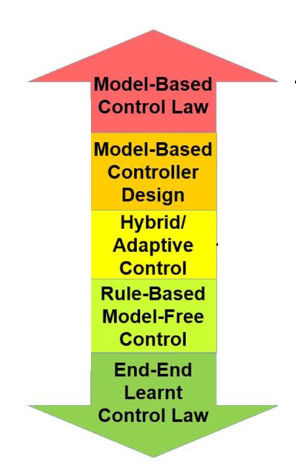
\includegraphics[width=0.2\textwidth]{img02.png}
	\captionsetup{width=0.6\linewidth}
	\caption{The continuum in the literature in regards to control
		methodology ranging from model-based to end-end data-driven
		control \cite{thakar2023survey}}
	\label{fig:img02}
\end{figure}


\textbf{\textit{Mobile Manipulator for Autonomous Localization,
		Grasping and Precise Placement of Construction
		Material in a Semi-Structured Environment}} \quad
A starting point for mobile manipulation is the work \cite{loianno2021construction},
presenting the winning mobile manipulation system for the \textit{Mohamed
	Bin Zayed International Robotics Challenge (MBZIRC)} held in 2020. The proposed system
is comprised of a mobile wheeled base performing localization and navigation in a
semi-structured environment, and a 5-DoF manipulator for grasping and precise placement
of bricks in a carrier. This work was among the first to demonstrate the potentialities
in mobile manipulation in a practical scenario.

%add img13 from the paper
\begin{figure}[H]
	\centering
	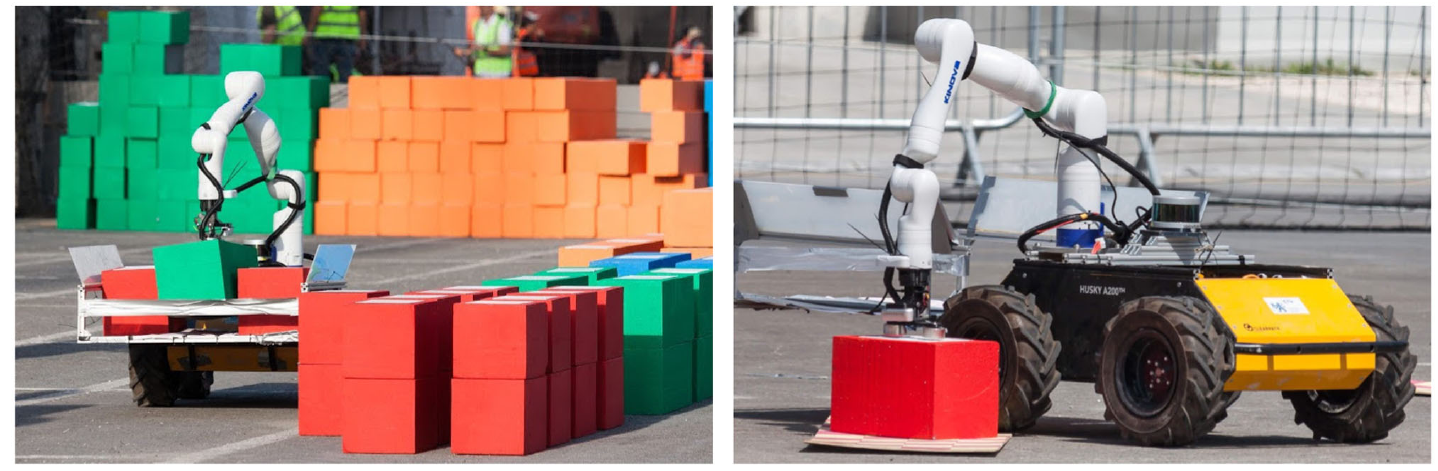
\includegraphics[width=1\textwidth]{img13.png}
	\captionsetup{width=1\linewidth}
	\caption{The described system loading and placing building material
		during the MBZIRC 2020 contest.	\cite{loianno2021construction}}
	\label{fig:img13}
\end{figure}

However, their approach is based on many simplyfying assumptions which may be suitable as a
first one of a kind robotic pick and place system in a real-world scenario and application,
but is not robust enough for a more complex task. For example, the grasping pipeline
is trained to handle only bricks, i.e. solid parallelepiped objects, for which the grasping pose
is straightforward to compute. Furthermore, the robot is not able to autonomously decide
where to place the brick, but it is only able to place it in the predefined position.
Also the arm controller is quite primitive, since it doesn't handle the self collisions
appropriately, and the arm is not able to avoid obstacles in its workspace.

\textbf{\textit{Go Fetch: Mobile Manipulation in Unstructured Environments}} \quad
This work \cite{blomqvist2020gofetch} presents a mobile manipulation system
that combines perception, localization, navigation,
motion planning and grasping skills into one common workflow
for fetch and carry applications in unstructured indoor environments. 
The integration across the various modules is experimentally demonstrated 
in the video \cite{youtube2020gofetch} on the task of finding a commonly available 
object in an office environment, grasping it, 
and delivering it to a desired drop-off location. 

%add img16 from the paper
\begin{figure}[H]
	\centering
	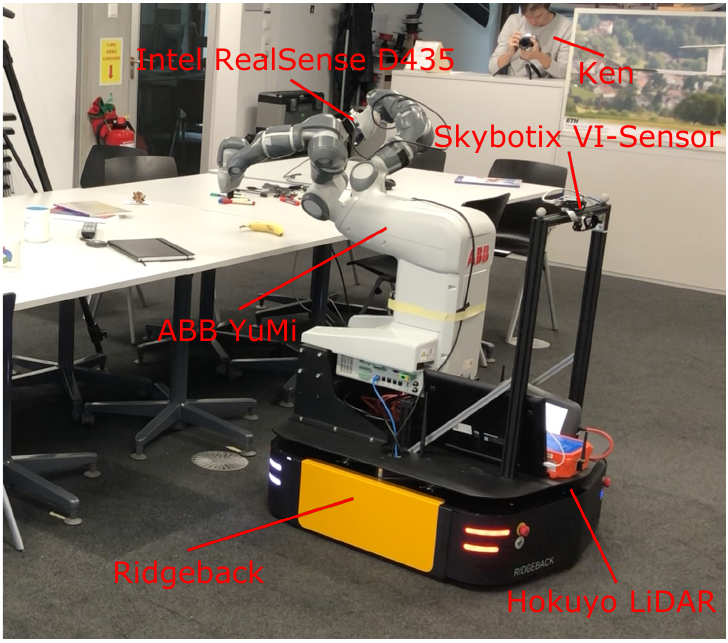
\includegraphics[width=0.6\textwidth]{img16.png}
	\captionsetup{width=0.8\linewidth}
	\caption{A picture of RoyalYumi in action. It features a two-arm ABB Yumi, a Clearpath 
	Ridgeback mobile base, two Hokuyo 2D LiDARs, an	Intel RealSense D435 and a Skybotix VI-Sensor.
	\cite{blomqvist2020gofetch}}
	\label{fig:img16}
\end{figure}

The research \cite{blomqvist2020gofetch} is an example of a mobile manipulation system
for pick and place task in an indoor environment that adopted many simplifications in order
to achieve the desired results. The system uses a series of heuristics to perform the
approaching to the object and the grasping phase, as it can be seen from the demonstration video
\cite{youtube2020gofetch}. The navigation uses a feature-based map and localization
modules, while the arm controller is handled by MoveIt! \cite{moveit2} solver coupled with
the ROS framework \cite{ros2}. This system is not very
well integrated as each phase of the task is carried out by a different module, and shows
how slow and inefficient the robot is in picking the banana. The grasping phase uses multiple
views of the object in order to compute a better grasp pose, which works well
but seems to be overly complex given the predefined task. Overall, the system 
can be regarded as a starting point for mobile manipulation and one of the first
works in dual-arm manipulability.

\subsection{Deep Reinforcement Learning - Data Driven Approach}

Explicit programming is often needed in practice to account for uncertainties in the environment and
sensors used, as well as to solve highly variable problems in an efficient way.
Explicit behavior programming is therefore often tedious and impractical, and more flexible solutions
are needed in environments where the robot must adapt to.
Alternatively, data-driven approaches address the main limitations of traditional methods and propose
to learn robotic behaviours from real experience, thus alleviating the cost of modelling complex behaviours.
This approach allows them to use deep neural networks to model the uncertainties of the environment,
which leads to a more robust controller compared to traditional ones.
Unlike deep learning (DL), the reinforcement learning (RL) paradigm allows to automatically obtain the
experience needed to learn robotic skills through trial-and-error and allows to learn complex decision-making
policies.

With RL, the explicit modelling of the problem is no longer required since the learnt models are grounded
in real experience. Recently, the combination of DL and RL, also known as Deep Reinforcement Learning (DRL),
has made it possible to tackle complex decision-making problems that were previously unfeasible. It combines
the ability of DL to model very high dimensional data with the ability of RL to model decision-making agents
through trial and error.
In fact, DRL has proven to be the state-of-the-art technology for learning complex
robotic behaviours through the interaction with the environment and solely guided
by a reward signal \cite{liu2021deep}.

While ML-based methods are generally used for offline forecasting, DRL is generally used online in
sequential decision-making problems. In fact, DRL allows to autonomously learn complex control policies
through trial and error and only guided by a reward signal. In the case of robotics, the most common
use case is to use such algorithms to model agents capable of performing continuous control of robots.

DRL has been successfully applied in a wide variety of areas such as robotics, computer vision and gaming.
Taking into account the difficulty of modelling complex decision-making robotic skills, DRL offers
a promising way to take advantage of the experience gathered interacting with the environment to
autonomously learn complex robotic behaviours. In particular, the field of DRL applied to robotics has
recently gained popularity due to the remarkable performance obtained in applications 
with high decision-making and control complexity. 
Applications range from manipulation, to autonomous navigation and locomotion.
\cite{iriondo2023learning}

\begin{figure}[H]
	\centering
	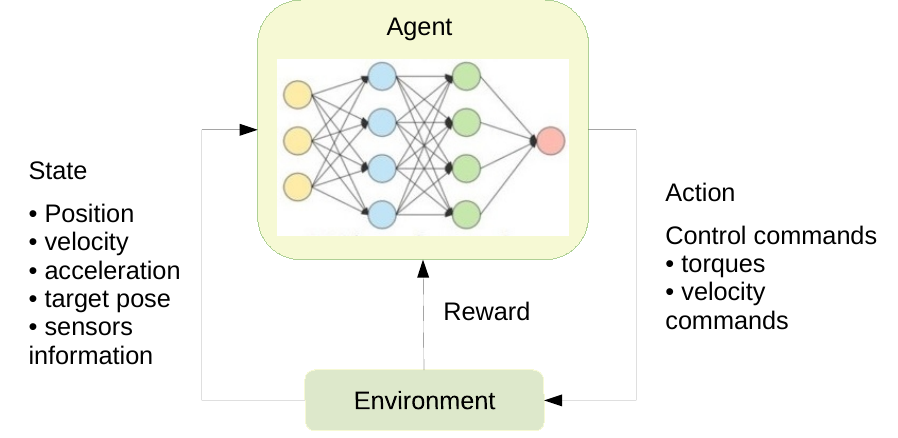
\includegraphics[width=0.7\textwidth]{img03.png}
	\captionsetup{width=0.8\linewidth}
	\caption{A schematic diagram example for robotic manipulation control
		using a data-driven approach such as DRL \cite{liu2021deep}}
	\label{fig:img03}
\end{figure}

\textbf{\textit{Pick and Place Operations in Logistics Using
a Mobile Manipulator Controlled with Deep
Reinforcement Learning}} \quad
The work \cite{iriondo2019pickandplace} presents one of the first and pioneering approaches
to DRL-based methods for pick and place tasks. Their work focused on the positioning
problem, consisting in a local navigation problem where the robot must move to a desired
position moving by small distances in a confined environment to reach the target object.
They relied on DRL for controlling the mobile wheeled base robot, while the arm controller
was handled by MoveIt! framework \cite{moveit2}. This can be regarded as a first step towards
more complex tasks, as it shows the foundations of DRL-based methods for mobile manipulation.
The method had some flaws, like the imprecise navigation due to errors in localization and
odometry, which the network was not able to overcome, since it was not fed video data stream.
However, it paved the wasy for a lot of other works, many of which mentioned in this chapter.

\textbf{\textit{Fully Autonomous Real-World Reinforcement
		Learning with Applications to Mobile Manipulation}} \quad
A work from Berkeley AI research \cite{sun2022relmm} show \textit{ReLMM}, a model that
can learn continuously on a real-world platform without any environment instrumentation,
without human intervention, and without access to privileged information, such as maps,
objects positions, or a global view of the environment. Their method employs a
modularized policy with components for manipulation and navigation, where manipulation
policy uncertainty drives exploration for the navigation controller, and the manipulation
module provides rewards for navigation. They trained the policy on a room cleanup task, where
the robot must navigate to and pick up items scattered on the floor.
The robot learns entirely from its own sensors in a real-world environment, without any
simulation and minimal human intervention. Furthermore, the entire learning process is efficient
enough for real-world training. On top of this, the robot is able to continually gather data
at scale and improve its performance over time, with the auto-reset functionality.

%add img11 from the paper
\begin{figure}[H]
	\centering
	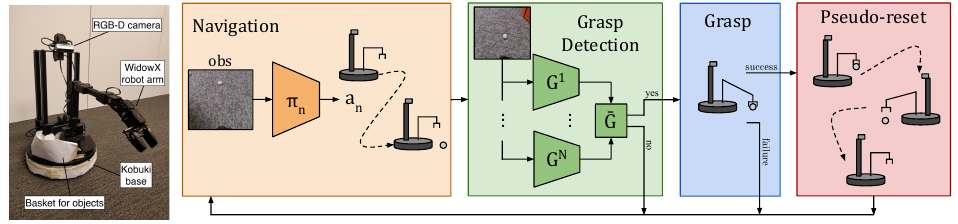
\includegraphics[width=1\textwidth]{img11.png}
	\captionsetup{width=1\linewidth}
	\caption{ReLMM partitions the mobile manipulator into a navigation policy
		and grasping policy. Both policies are rewarded when an object is grasped
		\cite{sun2022relmm}}
	\label{fig:img11}
\end{figure}

Although the results shown in \cite{sun2022relmm} demonstrate efficient performance in
the pick and place task, there are many issues circumvented by simplyfying the problem.
For example, the robot is very small, a modified version of Turtlebot, running in a small and
contained environment. They didn't address any safety and collision issues since the platform
mounted bumping sensors, and any collision would not harm the robot at all. Doing so enabled them
to train the policy online without any prior simulation.
Furthermore the kinematics of the mobile base and the robotic arm are very simple, and having the
stereo camera mounted on top of the robotic platform allowed them to easily detect the objects
on the floor. This work paves the way for more complex systems and tasks, but it is still far
from being a general solution for mobile manipulation.

\subsection{Challenges in Data-Driven approaches}

Two of the most important challenges here concern \textbf{sample efficiency and generalization}.
The goal of DRL in the context of robotic manipulation
control is to train a deep policy neural network, to detect the optimal
sequence of commands for accomplishing the task. The current state of the algorithm can include
the angles of joints of the manipulator, position of the end effector, and their derivative information,
like velocity and acceleration. The output of this policy network is an action indicating control
commands to be implemented to each actuator, such as torques or velocity commands. When the robotic manipulator
accomplishes a task, a positive reward will be generated. With these delayed and weak
signals, the algorithm is expected to find out the most successful control strategy for the
robotic manipulation \cite{liu2021deep}.

The challenges of learning robust and versatile manipulation skills
for robots with DRL are still far from being resolved satisfactorily for real-world application.
Currently, robotic manipulation control with DRL may be suited to fault tolerant
tasks, like picking up and placing objects, where a disaster will not be caused if the
operation fails occasionally. It is quite attractive in situations, where there is enough
variation that the explicit modeling algorithm does not work \cite{liu2021deep}.

However, even in this kind of applications, DRL-based methods are not widely
used in real-world robotic manipulation. The reasons are multiple, including sample efficiency and generation,
where more progress is still required, as both gathering experiences by interacting with
the environment and collecting expert demonstrations for imitation learning are expensive
procedures, especially in situations where robots are heavy, rigid and brittle, and it will
cost too much if the robot is damaged in exploration. Another very important issue is
\textbf{safety guarantee}. Not like simulation tasks, we need to be very careful that learning
algorithms are safe, reliable and predictable in real scenarios, especially if we move to
other applications that require safe and correct behaviors with high confidence, such as
surgery or household robots taking care of the elder or the disabled. There are also other
challenges including but not limited to the algorithm explainability, the learning speed,
high-performance computational equipment requirements. \cite{liu2021deep}

\textbf{\textit{Learning positioning policies for mobile manipulation operations
		with deep reinforcement learning}}
\quad
The work proposed in \cite{iriondo2023learning} is a practical example of a DRL-based approach
facing these challenges and the enormous limitations to overcome (as well as the potentialities).
The mobile platform in figure \ref{fig:img01} is used in an industrial environment for an
approaching task. The robot learns to navigate itself to the desk where the target object is located,
then uses the MoveIt! planner to check whether the trajectory to pick the object is feasible.
The robot locates itself using AMCL and the learned policy serves as a controller for
local navigation task. Their work show many shortcomings of this approach, such as the
difficult integration between the DRL policy and localization package, with noise in the
real environment affecting negatively the performance of the robot. As a result,
the video presented shows an inefficient an jiggly movement
because of the non-smooth control policy. In fact, they mention the necessity of mounting
a stereo camera for navigation, in order to reduce the errors in the localization and
improve the navigation of the robot.


\begin{figure}[H]
	\centering
	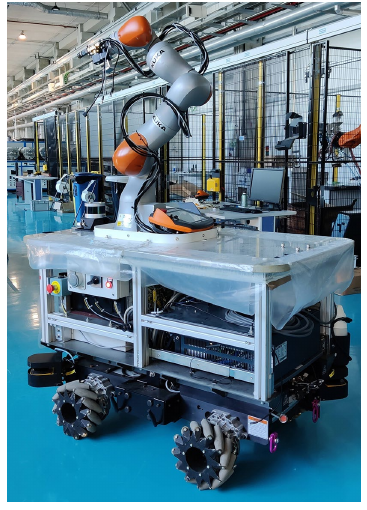
\includegraphics[width=0.5\textwidth]{img01.png}
	\captionsetup{width=0.6\linewidth}
	\caption{KUKA robot mounted on a mobile platform for pick and place tasks
		in industrial environments \cite{iriondo2023learning}}
	\label{fig:img01}
\end{figure}



\textbf{\textit{Deep Reinforcement Learning Based Mobile Robot Navigation Using Sensor Fusion}} \quad
The problem of unstable and imprecise navigation with learned policies is overcome in the
paper \cite{yan2023drlnavigation}, which proposes a DRL-based approach for navigation in dynamic
environments. The proposed method is based on the Deep Deterministic Policy Gradient (DDPG)
algorithm, which is a model-free, off-policy actor-critic algorithm that uses deep neural networks
to represent the policy and the critic functions. The proposed method is evaluated in a
simlated environment where the robot learns to navigate effectively and smoothly, while avoiding
unknown dynamic obstacles. This work shows the right direction towards more robust
navigation and obstacle avoidance systems.

\section{Whole-body mobile manipulator control}

In most control approaches to mobile manipulation, base and manipulator operation are strictly
separated such that at any given time only one primary control objective is
active. This separation principle is then augmented by a switching layer that determines the
currently pertinent control objectives. The advantage of such a control formulation lies in its
implicity, i.e., priorities can be separated among the arm and the base with individually
designed different control algorithms employed for each subsystem \cite{thakar2023survey}.

Instead, we refer to \textbf{whole-body control} as a unified control framework that considers
the mobile manipulator as a single system (arm manipulator mounted on a mobile wheeled/legged robot).
Despite the disadvantage that unified control needs to adhere to a single control framework,
it allows for the exploitation of mobile manipulation in the true sense of the term,
wherein the manipulator and mobile base can be controlled at the same time. This can lead
to several advantages during task achievement and makes the robot more dynamic in terms
of its capabilities. The formulation for this type of control involves considering
the onboard manipulator as an extended joint space of the mobile base, where the motion controller
considers both the base and manipulator state. As a result, base control can be completed
simultaneously without affecting much the performance of the end-effector manipulability
\cite{thakar2023survey}.

\subsection{MPC+IK for articulated object manipulation}

\textbf{\textit{Articulated Object Interaction in Unknown Scenes
		with Whole-Body Mobile Manipulation}} \quad
In a work conducted in universities in Zurich and Toronto \cite{mittal2022articulated},
the researchers demonstrated a successful application of whole-body control for a mobile
manipulator. The proposed system introduces a two-stage architecture for autonomous interaction
with large articulated objects in unknown environments.

%add image from the paper
\begin{figure}[H]
	\centering
	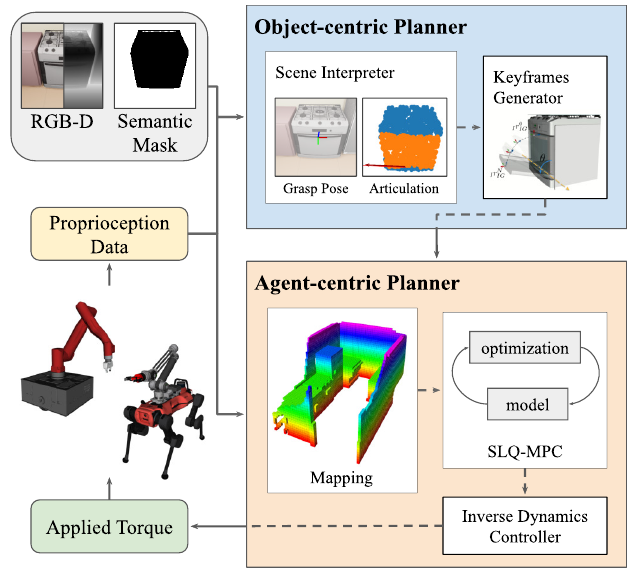
\includegraphics[width=0.7\textwidth]{img04.png}
	\captionsetup{width=0.9\linewidth}
	\caption{ The two-level hierarchy in the proposed framework. The
		object-centric planner comprises of a scene interpreter and keyframe
		generator. It uses perceptual information to generate task space
		plans. The agent-centric planner follows the computed plan while
		satisfying constraints and performing online collision avoidance.
		\cite{mittal2022articulated}}
	\label{fig:img04}
\end{figure}


In the first stage, an object-centric planner focuses solely on the object, providing an
action-conditional sequence of states for manipulation using RGB-D data.
The second stage involves an agent-centric planner that formulates whole-body motion control
as an optimal control problem, ensuring safe tracking of the generated plan, even in scenes
with moving obstacles.
The system proposed in \cite{mittal2022articulated} demonstrates effectiveness in handling complex static and
dynamic kitchen settings for both wheel-based and legged mobile manipulators. A comparison with
other agent-centric planners reveals a higher success rate and lower execution time. Hardware
tests on a legged mobile manipulator further confirm the system's capability to interact with
various articulated objects in a real kitchen. The approach combines object-centric and
agent-centric planning, leveraging MPC-based solutions for improved success rates and reduced
execution times, particularly in articulated object manipulation scenarios. The contributions
include the extension of collision-free whole-body MPC for mobile manipulation, benchmarking
in hyper-realistic simulation, and successful hardware experiments showcasing the system's
real-world applicability.


%add image from the paper
\begin{figure}[H]
	\centering
	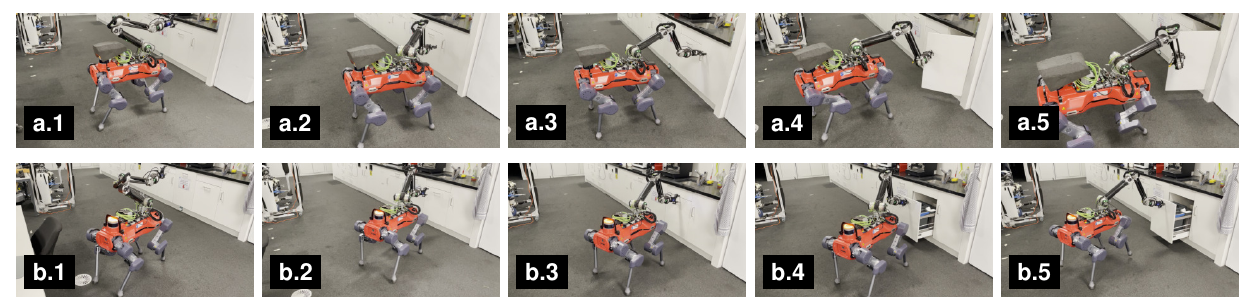
\includegraphics[width=1\textwidth]{img05.png}
	\captionsetup{width=1\linewidth}
	\caption{Legged mobile manipulation of articulated objects in the kitchen test scenario:
		(a) Drawer, (b) Cabinet. Throughout the interaction, we set the robot gait schedule
		to trot. Only while grasping the handle, the robot enters stance mode.
		\cite{mittal2022articulated}}
	\label{fig:img05}
\end{figure}


The work \cite{mittal2022articulated}, published in 2022, is the first and one of a kind
in successful real-world application of whole-body control using a MPC-based approach
combined with IK solvers for articulated object manipulation.
Furthermore, they achieved good performance in both dynamic
and static real world environments, which is a very challenging task for most of the
existing methods. However, the proposed method is limited mostly with respect to the grasping
capabilitities, which were hard-coded into the known interactive objects (in their case,
the kitchen appliances handles), meaning that explicit behavior programming and tuning was
needed for the grasping task. They propose data-centric methods to overcome these limitations.
This research proved the feasibility of this approach, which many other researchers claimed
to be unfeasible and way too complex to be implemented in real-world applications. However,
it is worth noting that the proposed method is not a general solution for all robots hardware
configurations, and extending it to other robots would require a lot of effort and time,
since it boils down to an optimal control problem.

\subsection{Deep Reinforcement Learning for high DoF control}

\textbf{\textit{Deep Whole-Body Control: Learning a Unified Policy
		for Manipulation and Locomotion}} \quad
The research paper \cite{fu2022deeplegged} addresses the challenges in controlling legged
manipulators with attached arms, proposing a novel approach to learn a unified policy for
whole-body control using deep reinforcement learning. The standard hierarchical control pipeline
is critiqued for its inefficiency, requiring significant engineering to coordinate
arm and leg movements. The proposed method, Regularized Online Adaptation, aims to bridge the Sim2Real gap,
and Advantage Mixing is introduced to overcome local minima during training.
The authors present a low-cost legged manipulator design and demonstrate that their
unified policy enables dynamic and agile behaviors across various tasks.

%add image from the paper
\begin{figure}[H]
	\centering
	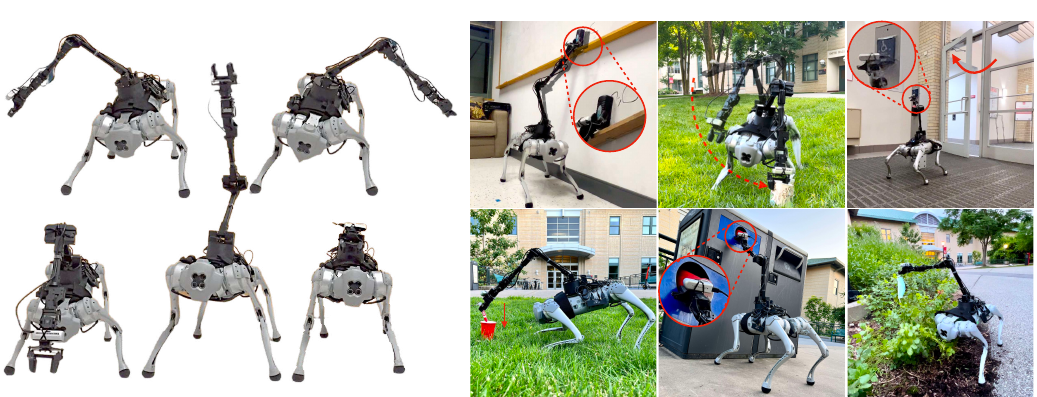
\includegraphics[width=1\textwidth]{img06.png}
	\captionsetup{width=1\linewidth}
	\caption{Framework for whole-body control of a legged robot with a robot arm attached.
		Left half shows how whole-body control achieves larger workspace by leg bending and stretching.
		Right half shows different real-world tasks, including wiping whiteboard, picking up a cup,
		pressing door-open buttons, placing, throwing a cup into a garbage bin and picking
		in clustered environments. \cite{fu2022deeplegged}}
	\label{fig:img06}
\end{figure}

The paper emphasizes the limitations of current hierarchical models, advocating for learning-based
methods like reinforcement learning to reduce engineering efforts and improve generalization.
However, it critiques existing learning-based approaches for semi-coupling legs and arms,
highlighting issues of coordination, error propagation, and non-smooth motions.
The proposed unified policy not only allows coordination but also enhances the capabilities
of individual components, such as the robot dynamically adjusting leg movements to extend
the arm's reach \cite{fu2022deeplegged}.

The challenges in scaling standard sim2real reinforcement learning to whole-body control
are discussed, including the high degree of freedom, conflicting objectives, and dependencies
between manipulation and locomotion. The paper introduces a hardware setup for a low-cost, fully
untethered legged manipulator and outlines a method for learning a unified policy to control
both legs and the arm. The authors leverage causal structure in action space and regularization
for domain adaptation to enhance stability and speed up learning.
The proposed method is evaluated through tasks like teleoperation and vision-guided tracking,
demonstrating successful picking tasks using visual feedback from an RGB camera.
Comparative analysis with a baseline method (MPC+IK) across various pick-up tasks measures success rate,
average time to completion, IK failure rate, and self-collision rate.
The authors conclude by acknowledging the preliminary nature of their results and highlight
potential extensions, such as incorporating vision-based policies and addressing challenges
in general-purpose object interaction \cite{fu2022deeplegged}.

%add image from the paper
\begin{figure}[H]
	\centering
	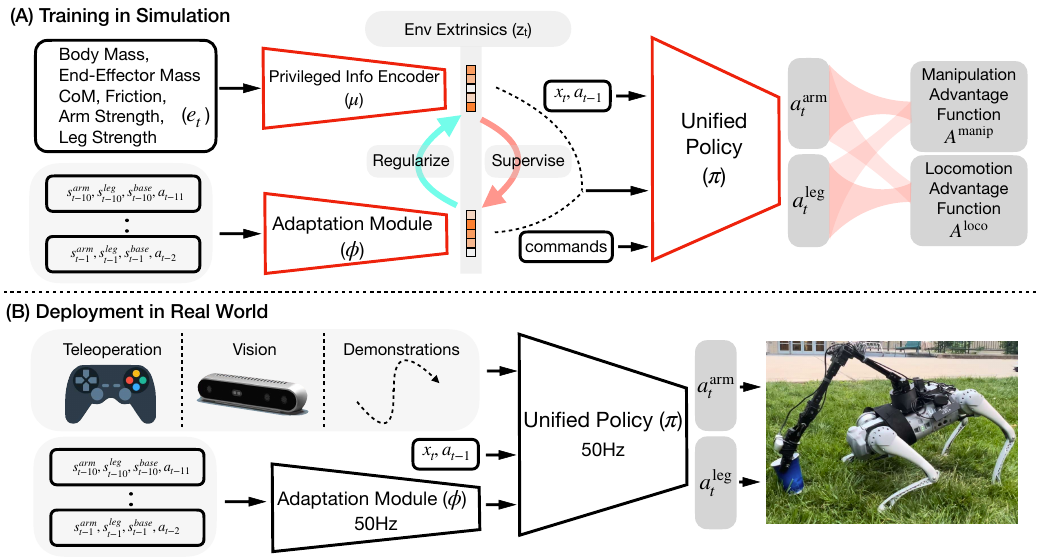
\includegraphics[width=1\textwidth]{img07.png}
	\captionsetup{width=1\linewidth}
	\caption{Whole-body control framework. During training, a unified policy is learned by conditioned on
		environment extrinsics. During deployment, the adaptation module is reused without
		any real-world fine-tuning.
		The robot can be commanded in various modes including teleoperation, vision and demonstration replay.
		\cite{fu2022deeplegged}}
	\label{fig:img07}
\end{figure}

As the authors of the paper \cite{fu2022deeplegged} state, the main limitation (but also the core
idea behind the control input) is the fact that the robot requires a human operator to
provide the robot objectives, which are then translated into the control inputs. In fact,
the robot is not able to autonomously decide what to do, but it is only able to either track the
end effector pose given by the human operator, or to track the April marker in the human's hand.
This limitation can be overcome with appropriate task training, but it is not a general solution.
However, the proposed method is very promising, since it is able to achieve very good results
in the robot body-hand coordination, which is a very challenging task for most of the existing
methods. The movements look very smooth and natural, and the robot is able to perform
simple task in dynamic environment. The April marker tracking mode shows also the effectiveness of
the use of a stereo camera for tracking the objective, meaning that promising results can be
achieved in other tasks. This research used Isaac Gym as a simulation environment, which
proved to be very powerful for training and overcoming the simulation-to-reality gap.

\textbf{\textit{Learning Mobile Manipulation through Deep
		Reinforcement Learning}} \quad
\cite{wang2020drlmanipulation}
This paper presents a pioneering mobile manipulation system that leverages deep
reinforcement learning for unstructured environments. It uniquely integrates state-of-the-art
algorithms with visual perception, adopting an efficient framework that separates
visual processing from control. This design enables seamless generalization from simulation
training to real-world scenarios, utilizing only on-board sensors.
Notably, the transferability of policies from simulation to real robots is a key strength,
demonstrating the system's autonomy in grasping diverse objects across varied scenarios.
The evaluation centers around a challenging mobile picking task, encompassing object recognition,
collision-free robot-arm control, and object picking based on the learned policy.


%add img14 from the paper
\begin{figure}[H]
	\centering
	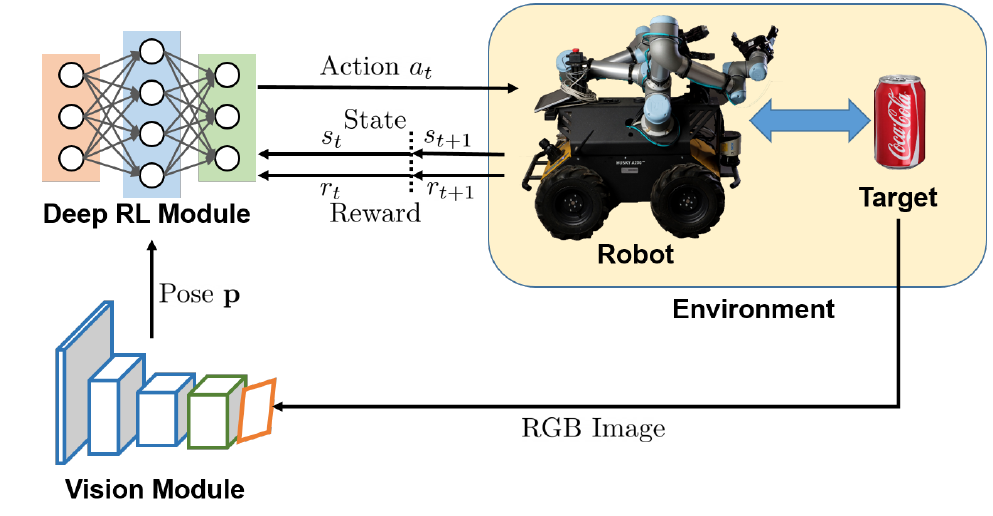
\includegraphics[width=1\textwidth]{img14.png}
	\captionsetup{width=1\linewidth}
	\caption{Learning-based mobile manipulation control framework. There are mainly two parts,
		deep reinforcement learning module and vision module. First, the vision module estimates
		the object 6-degrees of freedom pose $p$ from images captured by an on-board RGB stereo camera.
		Then, based on the object pose $p$ and current robot state st, deep reinforcement learning
		module predicts an action at for the robot to act. A new state $s_{t+1}$ and a reward
		$r_{t+1}$ are received after action.\cite{wang2020drlmanipulation}}
	\label{fig:img14}
\end{figure}

Comparative assessments with state-of-the-art reinforcement learning algorithms highlight
the stability and efficacy of the Proximal Policy Optimization (PPO) based system.
Real-world experiments further confirm the system's ability to autonomously execute mobile grasping,
overcoming challenges posed by the intricate nature of mobile base, arm, gripper, and vision subsystems.
Acknowledging differences between simulation and real-world dynamics, the paper addresses
the need for closer coupling between mobile base and arm motions in future work. Overall,
this work represents a significant contribution to the field, showcasing the potential of
deep reinforcement learning for autonomous mobile manipulation in complex, unstructured environments.

%add img15 from the paper
\begin{figure}[H]
	\centering
	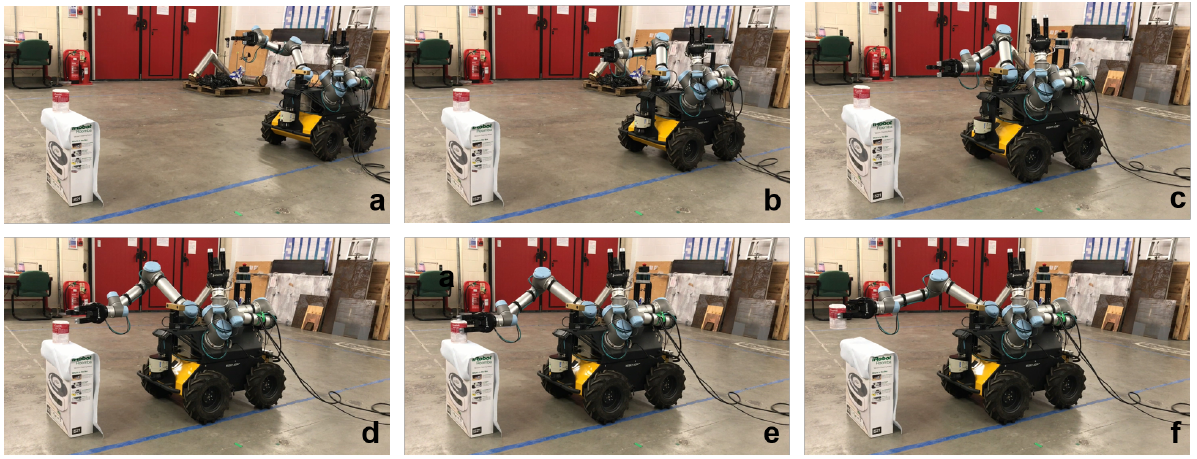
\includegraphics[width=1\textwidth]{img15.png}
	\captionsetup{width=1\linewidth}
	\caption{Real mobile grasping process for a soup can.
	(a) is starting, (b,c,d) is approaching, (e) is grasping, (f) is picking up.
	\cite{wang2020drlmanipulation}}
	\label{fig:img15}
\end{figure}

The method proposed in \cite{wang2020drlmanipulation} is very promising, since it is able to
achieve very good results in the robot body-hand coordination, which is a very challenging task
especially in dynamic environments. The movements look very smooth and natural, and the robot is
able to perform simple task in dynamic environment. This approach is one of the first able
to achieve such complex control using vision-based perception together with deep reinforcement
learning. However, it is far from being an optimal solution, since it achieves simple
tasks in a very controlled environment. The research paper mentioned below is from the same
research group, demonstrating the new advancements in their research.

\textbf{\textit{Multi-Task Reinforcement Learning based Mobile Manipulation 
	Control for Dynamic Object Tracking and Grasping}} \quad
This research paper \cite{wang2022multitask} is a continuation of work demonstrated in the
their previous research paper \cite{wang2020drlmanipulation} mentioned above.
\cite{wang2022multitask} addresses the challenges associated with
agile control of mobile manipulators in unstructured environments, particularly focusing
on dynamic object tracking and grasping. The authors propose a multi-task reinforcement
learning-based control framework that aims to achieve general dynamic object tracking and
grasping capabilities. The framework utilizes various dynamic trajectories as a training set,
incorporating random noise and dynamics randomization to enhance policy generalization.
Experimental results demonstrate the trained policy's ability to adapt to unseen dynamic
trajectories, achieving a 0.1m tracking error and a 75\% grasping success rate for dynamic objects.
The proposed method is successfully deployed on a real mobile manipulator, showcasing its
potential for real-world applications. The contributions of this work include the development
of a versatile control framework and its successful deployment in unstructured environments,
addressing the challenges of mobile manipulation with dynamic objects.

%add image from the paper
\begin{figure}[H]
	\centering
	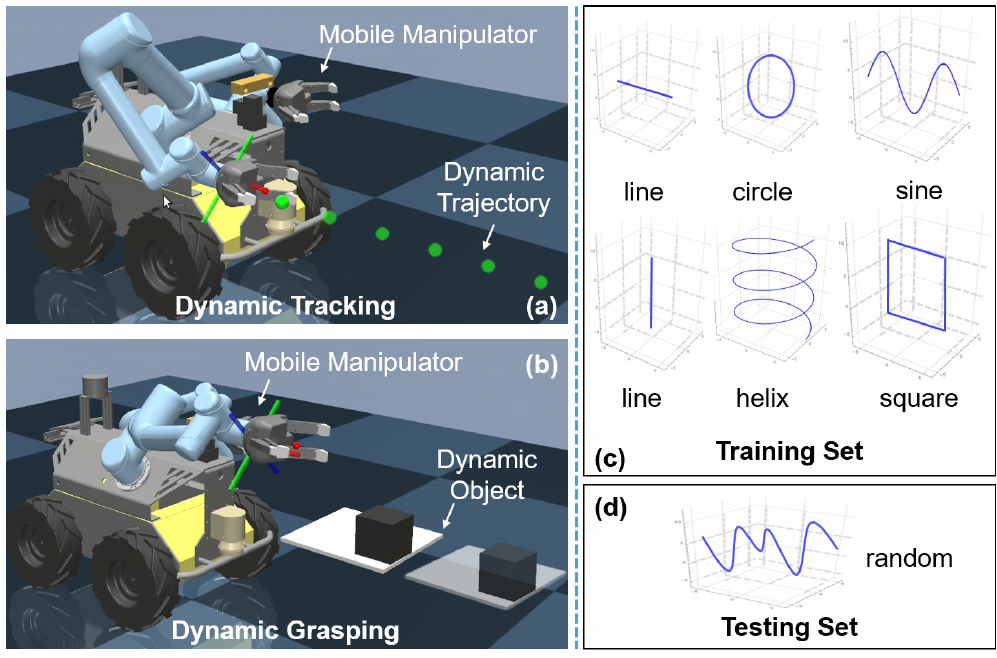
\includegraphics[width=1\textwidth]{img08.png}
	\captionsetup{width=1\linewidth}
	\caption{(a) Dynamic trajectory tracking task with a mobile manipulator. (b)
		Dynamic object grasping task with a mobile manipulator. (c) Several basic
		trajectories as multi-task RL training set. (d) Random trajectories as multi-task
		RL testing set.\cite{wang2022multitask}}
	\label{fig:img08}
\end{figure}

In \cite{wang2022multitask} they use the proximal policy optimization (PPO) algorithm to train
and learn a policy, but the method is general and can be applied to most on/off-policy RL algorithms.
PPO is one of the state-of-the-art RL algorithms that is easy to implement and tune, and performs
relatively well. The policy is learned through a deep neural network.

%add image from the paper
\begin{figure}[H]
	\centering
	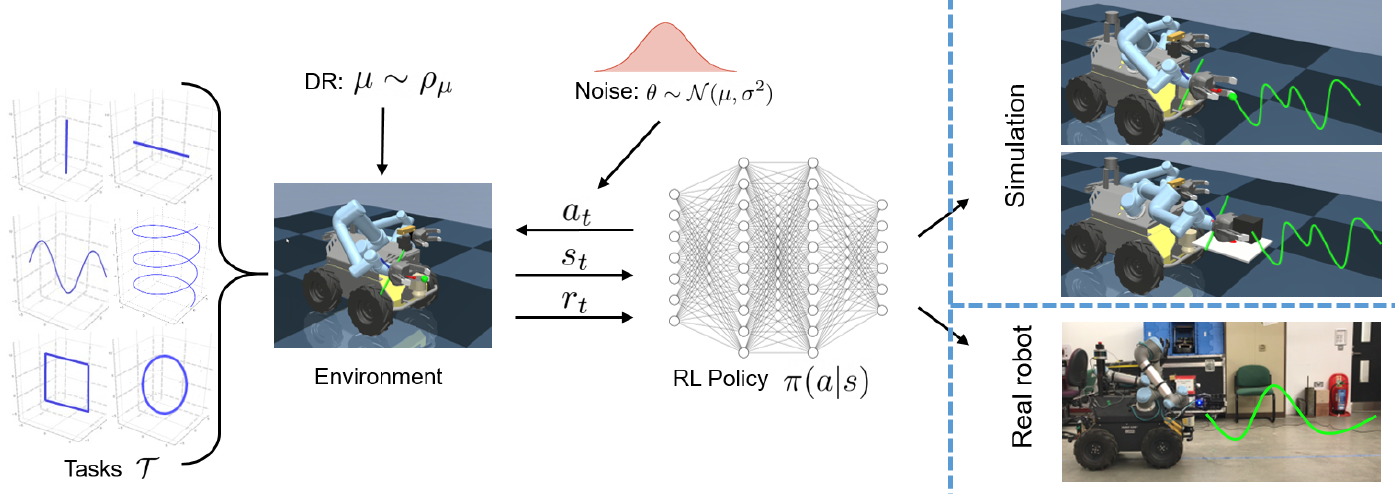
\includegraphics[width=1\textwidth]{img09.png}
	\captionsetup{width=1\linewidth}
	\caption{(a) In the multi-task RL training, six basic trajectories are used as the task
		training set to train a general policy. To improve the robustness, gaussian noise is added
		to the action and observation space in each training episode. (b) The RL testing includes
		simulation and real world for policy evaluation.\cite{wang2022multitask}}
	\label{fig:img09}
\end{figure}

The images above show the training and testing process of the proposed method. They created a
realistic simulation environment which enabled efficient parallel training of the policy,
and simulation of the dynamic objects and tracking. They also managed to correctly transfer the
learned policy to the real robot, which is a very challenging task for most of the existing methods.
Artificial noise addition was essential for the training process, since it allowed the policy
to generalize better to unseen trajectories and environments.

%add image from the paper
\begin{figure}[H]
	\centering
	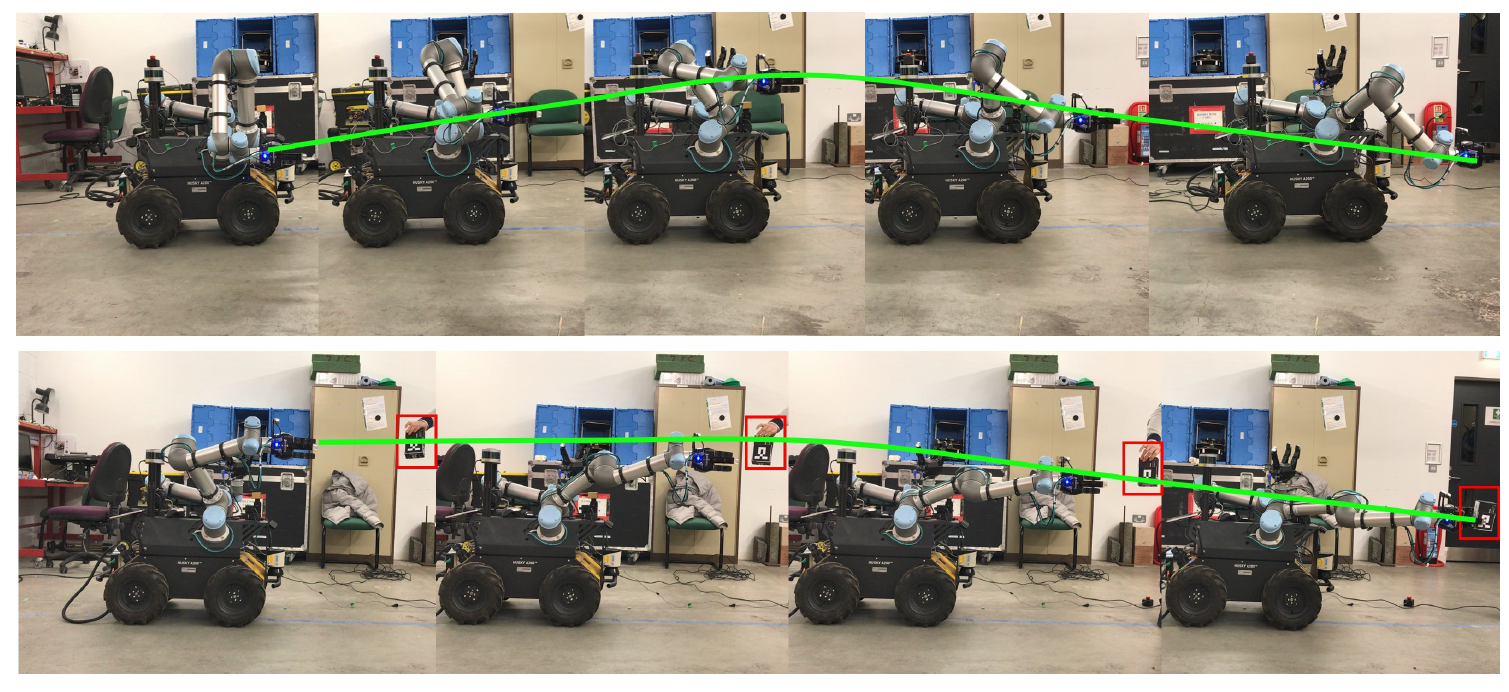
\includegraphics[width=1\textwidth]{img10.png}
	\captionsetup{width=1\linewidth}
	\caption{Snapshots of the real robot experiments. The upper row shows a mobile
		tracking process in which the end-effector try to track the target trajectory.
		The lower row shows a mobile grasping process in which the object moves
		randomly. \cite{wang2022multitask}}
	\label{fig:img10}
\end{figure}

Overall, this research provides valuable insights and a practical solution for advancing the
field of agile mobile manipulation. This is one of the very few works that addresses the
problem of dynamic object tracking and grasping, which is a very challenging task for most
of the existing models, due to the difficulty in modeling and the extensive training required. Although
the model doesn't show very high success rate in the tasks shown, it shows promising results
and a direction of research that can be further explored.



\subsection{Comparison of Model-Based and Data-Driven approaches}


\singlespacing
\begin{table}[H]
	\centering
	\begin{tabular}[c]{|m{3cm} || m{6cm} | m{6cm}|}
		\hline
		\raggedleft \textbf{Approach}                           &
		\textbf{Model-Based}                                    &
		\textbf{Data-Driven}
		\\
		\hline \hline

		\raggedleft \textbf{Control Strategies}                 &
		\customtablelist{
			\item Model Predictive Controllers (MPC)
			\item Whole-Body Inverse Kinematics (IK) Solver
		}                                                       &
		\customtablelist{
			\item Deep Reinforcement Learning (DRL)
			\item Imitation Learning
		}
		\\
		\hline

		\raggedleft \textbf{Features}                           &
		\customtablelist{
			\item Requires explicit modeling of system dynamics and kinematics
			\item Suitable for simple tasks, unsuitable for complex tasks
			\item Planning over end-effector pose or grasp in the workspace
		}                                                       &
		\customtablelist{
			\item No explicit modeling of system dynamics
			\item Learning from experience in simulation environments
			\item High-level planning over tasks, object detection, manipulation
			or other objectives
		}
		\\
		\hline

		\raggedleft \textbf{Interpret-ability and Adaptability} &
		\customtablelist{
			\item Explitic modeling implies high system interpretability
			\item Adaptable to many tasks but requires behaviors re-programming
		}                                                       &
		\customtablelist{
			\item Learned policies have very limited interpretability
			\item Learning from experience allows high adaptability,
			given proper GPU-parallelized training
		}                                                         \\
		\hline

		\raggedleft \textbf{Advantages}                         &
		\customtablelist{
			\item Small simulation-to-reality gap
			\item Adaptable to many tasks but with explicit programming
			\item No training required
			\item Safer operation due to explicit physical limitations modeling
		}                                                       &
		\customtablelist{
			\item No explicit modeling of system dynamics required
			\item Learning from experience allows high generalization
			\item Can perform well in unknown or dynamic environments
			\item Can provide high body-hand movement coordination
		}                                                         \\
		\hline

		\raggedleft \textbf{Disadvantages}                      &
		\customtablelist{
			\item Requires very accurate physical models for seamless integration
			\item Doesn't perform well in complex tasks or dynamic environments
			\item Difficult to adapt to complex tasks (low generalization)
			\item High computational cost for the solver in high DoF systems
		}                                                       &
		\customtablelist{
			\item Requires large amounts of training data and extensive training
			\item Very long time needed to fine tune the hyperparameters
			\item May result in unstable and jiggly movements
			\item May result in unsafe behaviors in real-world applications
			if not properly trained
			\item Suffers a lot from the simulation-to-reality gap
		}                                                         \\
		\hline
	\end{tabular}
	\caption{Summary of the main differences between model-based and data-driven approaches
		for robotic manipulator controls}
	\label{table:1}
\end{table}

\onehalfspacing


\section{Addressing the Simulation-to-Reality Gap}

\textbf{\textit{A Sim-to-Real Pipeline for Deep Reinforcement
		Learning for Autonomous Robot Navigation in
		Cluttered Rough Terrain}} \quad
A work from Toronto \cite{zhang2021simtoreal} proposes a sim-to-real pipeline for
deep reinforcement learning for autonomous robot navigation in cluttered rough terrain.
Sim-to-real strategies have been developed for robot navigation tasks. For example,
domain randomization can be applied to visual parameters such as texture,
lighting, and object placement in synthetic environments to improve the generalizability.
The paper \cite{zhang2021simtoreal} addresses the "sim-to-real Gap" in training robots for
3D terrain navigation by incorporating three sim-to-real strategies. Firstly, to account
for depth camera measurement errors in 3D mapping that affect terrain steepness accuracy,
the authors vary terrain steepness during training using a uniform distribution.
Secondly, the paper tackles disturbances in robot motion during interactions with rough
terrain, such as slippage and insufficient traction. Both 3D terrain interactions and
latency from visual odometry measurements contribute to disturbances in robot travel distance
and yaw rotation angle. The third strategy focuses on addressing robot pose estimation errors
arising from image and feature association errors. These errors, caused by lens distortion
and ambiguous features, impact the accuracy of the robot's estimated 6 DOF pose.
The paper integrates these errors into the inputs of the DRL network to improve the
model's performance in the face of localization inaccuracies.



\section{Object Detection and Grasping}

Grasp planning for mobile manipulators is a challenging problem that has been
dealt with in several ways in the literature. On the one hand, grasping requires coordination
within a very challenging high-dimensional constrained configuration space (mobile base /
manipulator / gripper). Further, grasping requires detecting object, constructing data-driven
representation, determining the gripper approach-vector, and computing all the mobile manipulator's
plans in the presence of uncertainty. Many of the traditional grasp planners (designed for stationary
manipulators) can be used for mobile manipulators once the mobile base has been fixed.
However, a generic grasping pipeline is desirable, which achieves arm-base-gripper
coordinated grasping given the information about object pose and
the operating environment. Such concurrent manipulator / mobile base motion approaches are being
explored till grasping is successful or at least until the gripper reaches the
objects (and only manipulator moves for grasping). This may not be optimal as grasping can happen
with the mobile base and the manipulator moving when the gripper is closing \cite{thakar2023survey}.

Broadly, automated grasping can be categorized into the following approaches 
\cite{asadi2019construction}: 

\begin{enumerate}
	\item grasp using prior information from scene/objects
	\item grasp using hand-eye coordination through learning directly from raw sensor data
	\item grasp using template matching
	\item grasp by detecting proper grasping pose using deep learning-based approaches
	\item other field-specific approaches
\end{enumerate}

Systems in each category have one or more limitations that are detailed in the following
subsections. The majority of the existing systems are static, where a robotic system 
is fixed in an environment surrounded by the objects in its workspace.

\textbf{\textit{Automated Object Manipulation Using Vision-Based Mobile 
Robotic System for Construction Applications}} \quad
The system designed and deployed for pick-and-place in a structured construction environment
\cite{asadi2019construction} integrates scene understanding and autonomous navigation 
with object grasping. To achieve this, two stereo cameras and a robotic arm are mounted
on a mobile platform. This integrated system uses a global-to-local control planning strategy
to reach the objects of interest (in this study, bricks, wood sticks, and pipes). 
Then, the scene perception, together with grasp and control planning, enables the system
to detect the objects of interest, pick, and place them in a predetermined location depending
on the application.
The system is implemented and validated in a construction-like environment for pick-and-place
activities. The results demonstrate the effectiveness of this fully autonomous system 
using solely onboard sensing for real-time applications with end-effector positioning
accuracy of less than a centimeter.
However, the researchers mention also the shortcomings of the system, since the robot
was developed for a field-specific application, therefore non-adaptable to more generic
use case scenarios. The system uses a heuristic-based approach in order to detect the
bricks to grasp and pick up. Furthermore, the navigation pipeline relies on a static environment
with no dynamic obstacles, since the arm manipulator does not employ any collision avoidance
in the trajectory planning \cite{asadi2019construction}.


\textbf{\textit{Autonomous Robotic Manipulation: Real-Time, Deep-Learning
		Approach for Grasping of Unknown Objects}} \quad
The work \cite{sayour2022unknowngrasping} proposes a novel approach for grasping unknown objects.
The researhers present a full grasping pipeline proposing a real-time data-driven
deep-learning approach for robotic grasping of unknown objects using MATLAB and
deep convolutional neural networks. The proposed approach employs RGB-D image data
acquired from an eye-in-hand camera centering the object of interest in the field of
view using visual servoing. Their approach aims at reducing propagation errors
and eliminating the need for complex hand tracking algorithm, image segmentation,
or 3D reconstruction, which are often either infeasible or too prone to errors.
The proposed approach is able to efficiently generate reliable multi-view object grasps
regardless of the geometric complexity and physical properties of the object in question.
The system employed is a 7 DoF robotic manipulator controlled with an IK solver,
and a parallel gripper with overactuated fingers.

%add img12 from the paper
\begin{figure}[H]
	\centering
	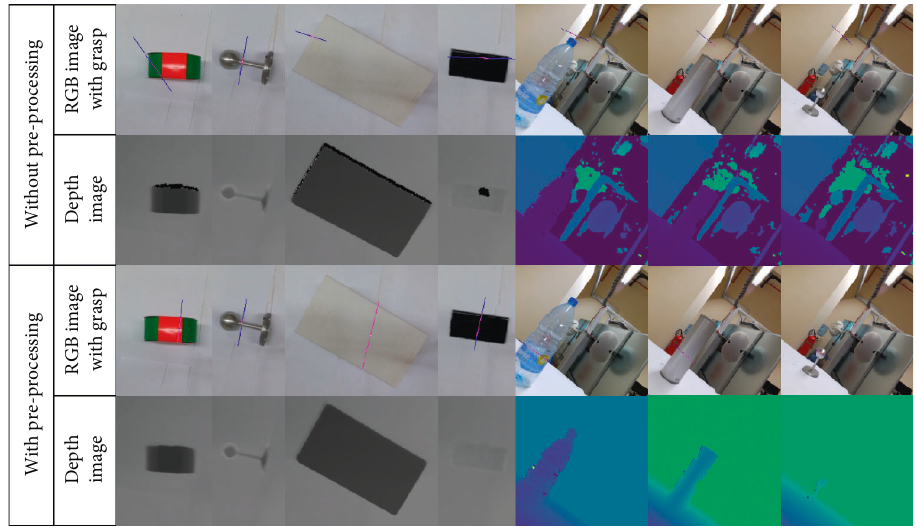
\includegraphics[width=1\textwidth]{img12.png}
	\captionsetup{width=1\linewidth}
	\caption{Grasp generation results: comparison between grasp generated by the GG-CNN
		with and without RGB-D image preprocessing for shiny and black objects
		\cite{sayour2022unknowngrasping}}
	\label{fig:img12}
\end{figure}

One of the main limitations of the approach in \cite{sayour2022unknowngrasping} is the fact
that the grasping pipeline is implemented in MATLAB, therefore hardly portable and hardly
replicable on other robotic hardware. Furthermore grasping with a parallel gripper is
very limited, and the approach can work well with a limited set of objects. The authors
demonstrated a good grasping capability with many different and unknown objects, but
the approach cannot be generalized well without creating a multi-view perspective of
the target object, in order to gain more understanding of the object's shape and
geometry. Although the approach is very promising, there is room for improvement,
especially in the CNN for grasping pose detection, which is the core of the grasping pipeline.


\TODO{add more papers about grasping?}


\section{Autonomous Exploration [todo?]}
